\documentclass{article}
\usepackage[margin=1in]{geometry}
\usepackage{hyperref}
\usepackage{amsmath,amsfonts,amssymb,amsthm,commath,dsfont}
\usepackage{enumitem}
\usepackage{framed}
\usepackage{xspace}
\usepackage{microtype}
\usepackage{float}
\usepackage[round]{natbib}
\bibliographystyle{plainnat}
\usepackage{cleveref}
\usepackage[dvipsnames]{xcolor}
\usepackage{graphicx}
\usepackage{listings}
\usepackage[breakable]{tcolorbox}
\tcbset{breakable}
\usepackage{mathtools}
\usepackage{caption}
\usepackage{subcaption}
\def\b1{\boldsymbol{1}}

\newcommand{\colbar}{\rule[-3mm]{.3mm}{1.5em}}
\newcommand{\rowbar}{\rule[.5ex]{1.5em}{.3mm}}
\DeclareMathOperator{\rank}{rank}
\def\balpha{\boldsymbol{\alpha}}
% following loops stolen from djhsu
\def\ddefloop#1{\ifx\ddefloop#1\else\ddef{#1}\expandafter\ddefloop\fi}
% \bbA, \bbB, ...
\def\ddef#1{\expandafter\def\csname bb#1\endcsname{\ensuremath{\mathbb{#1}}}}
\ddefloop ABCDEFGHIJKLMNOPQRSTUVWXYZ\ddefloop

% \cA, \cB, ...
\def\ddef#1{\expandafter\def\csname c#1\endcsname{\ensuremath{\mathcal{#1}}}}
\ddefloop ABCDEFGHIJKLMNOPQRSTUVWXYZ\ddefloop

% \vA, \vB, ..., \va, \vb, ...
\def\ddef#1{\expandafter\def\csname v#1\endcsname{\ensuremath{\boldsymbol{#1}}}}
\ddefloop ABCDEFGHIJKLMNOPQRSTUVWXYZabcdefghijklmnopqrstuvwxyz\ddefloop

% \valpha, \vbeta, ...,  \vGamma, \vDelta, ...,
\def\ddef#1{\expandafter\def\csname v#1\endcsname{\ensuremath{\boldsymbol{\csname #1\endcsname}}}}
\ddefloop {alpha}{beta}{gamma}{delta}{epsilon}{varepsilon}{zeta}{eta}{theta}{vartheta}{iota}{kappa}{lambda}{mu}{nu}{xi}{pi}{varpi}{rho}{varrho}{sigma}{varsigma}{tau}{upsilon}{phi}{varphi}{chi}{psi}{omega}{Gamma}{Delta}{Theta}{Lambda}{Xi}{Pi}{Sigma}{varSigma}{Upsilon}{Phi}{Psi}{Omega}{ell}\ddefloop

\newcommand\T{{\scriptscriptstyle\mathsf{T}}}
\def\diag{\textup{diag}}

\DeclareMathOperator*{\argmin}{arg\,min}
\DeclareMathOperator*{\argmax}{arg\,max}

\def\SPAN{\textup{span}}
\def\tu{\textup{u}}
\def\R{\mathbb{R}}
\def\E{\mathbb{E}}
\def\Z{\mathbb{Z}}
\def\be{\mathbf{e}}
\def\nf{\nabla f}
\def\veps{\varepsilon}
\def\cl{\textup{cl}}
\def\inte{\textup{int}}
\def\dom{\textup{dom}}
\def\Rad{\textup{Rad}}
\def\lsq{\ell_{\textup{sq}}}
\def\hcR{\widehat{\cR}}
\def\hcRl{\hcR_\ell}
\def\cRl{\cR_\ell}
\def\hcE{\widehat{\cE}}
\def\cEl{\cE_\ell}
\def\hcEl{\hcE_\ell}
\def\eps{\epsilon}
\def\1{\mathds{1}}
\newcommand{\red}[1]{{\color{red} #1}}
\newcommand{\blue}[1]{{\color{blue} #1}}
\def\srelu{\sigma_{\textup{r}}}
\def\vsrelu{\vec{\sigma_{\textup{r}}}}
\def\vol{\textup{vol}}
\def\sr{\sigma_r}


%%%%%%%%%%%%%%%%%%%%%%%%%%%%%%%%%%%%%%%%%%
% Custom commands                        %
%%%%%%%%%%%%%%%%%%%%%%%%%%%%%%%%%%%%%%%%%%
\newcommand{\blackcircle}{\tikz\draw[black,fill=black] (0,0) circle (1ex);}
\renewcommand{\circle}{\tikz\draw[black] (0,0) circle (1ex);}
% \newcommand{\vc}[1]{\boldsymbol{#1}}
\newcommand{\adj}[1]{\frac{d J}{d #1}}
\newcommand{\chain}[2]{\adj{#2} = \adj{#1}\frac{d #1}{d #2}}
\newcommand{\ntset}{test}

% mathcal
\newcommand{\Ac}{\mathcal{A}}
\newcommand{\Bc}{\mathcal{B}}
\newcommand{\Cc}{\mathcal{C}}
\newcommand{\Dc}{\mathcal{D}}
\newcommand{\Ec}{\mathcal{E}}
\newcommand{\Fc}{\mathcal{F}}
\newcommand{\Gc}{\mathcal{G}}
\newcommand{\Hc}{\mathcal{H}}
\newcommand{\Ic}{\mathcal{I}}
\newcommand{\Jc}{\mathcal{J}}
\newcommand{\Kc}{\mathcal{K}}
\newcommand{\Lc}{\mathcal{L}}
\newcommand{\Mc}{\mathcal{M}}
\newcommand{\Nc}{\mathcal{N}}
\newcommand{\Oc}{\mathcal{O}}
\newcommand{\Pc}{\mathcal{P}}
\newcommand{\Qc}{\mathcal{Q}}
\newcommand{\Rc}{\mathcal{R}}
\newcommand{\Sc}{\mathcal{S}}
\newcommand{\Tc}{\mathcal{T}}
\newcommand{\Uc}{\mathcal{U}}
\newcommand{\Vc}{\mathcal{V}}
\newcommand{\Wc}{\mathcal{W}}
\newcommand{\Xc}{\mathcal{X}}
\newcommand{\Yc}{\mathcal{Y}}
\newcommand{\Zc}{\mathcal{Z}}

% mathbb
\newcommand{\Ab}{\mathbb{A}}
\newcommand{\Bb}{\mathbb{B}}
\newcommand{\Cb}{\mathbb{C}}
\newcommand{\Db}{\mathbb{D}}
\newcommand{\Eb}{\mathbb{E}}
\newcommand{\Fb}{\mathbb{F}}
\newcommand{\Gb}{\mathbb{G}}
\newcommand{\Hb}{\mathbb{H}}
\newcommand{\Ib}{\mathbb{I}}
\newcommand{\Jb}{\mathbb{J}}
\newcommand{\Kb}{\mathbb{K}}
\newcommand{\Lb}{\mathbb{L}}
\newcommand{\Mb}{\mathbb{M}}
\newcommand{\Nb}{\mathbb{N}}
\newcommand{\Ob}{\mathbb{O}}
\newcommand{\Pb}{\mathbb{P}}
\newcommand{\Qb}{\mathbb{Q}}
\newcommand{\Rb}{\mathbb{R}}
\newcommand{\Sb}{\mathbb{S}}
\newcommand{\Tb}{\mathbb{T}}
\newcommand{\Ub}{\mathbb{U}}
\newcommand{\Vb}{\mathbb{V}}
\newcommand{\Wb}{\mathbb{W}}
\newcommand{\Xb}{\mathbb{X}}
\newcommand{\Yb}{\mathbb{Y}}
\newcommand{\Zb}{\mathbb{Z}}

% mathbf lowercase
\newcommand{\av}{\mathbf{a}}
\newcommand{\bv}{\mathbf{b}}
\newcommand{\cv}{\mathbf{c}}
\newcommand{\dv}{\mathbf{d}}
\newcommand{\ev}{\mathbf{e}}
\newcommand{\fv}{\mathbf{f}}
\newcommand{\gv}{\mathbf{g}}
\newcommand{\hv}{\mathbf{h}}
\newcommand{\iv}{\mathbf{i}}
\newcommand{\jv}{\mathbf{j}}
\newcommand{\kv}{\mathbf{k}}
\newcommand{\lv}{\mathbf{l}}
\newcommand{\mv}{\mathbf{m}}
\newcommand{\nv}{\mathbf{n}}
\newcommand{\ov}{\mathbf{o}}
\newcommand{\pv}{\mathbf{p}}
\newcommand{\qv}{\mathbf{q}}
\newcommand{\rv}{\mathbf{r}}
\newcommand{\sv}{\mathbf{s}}
\newcommand{\tv}{\mathbf{t}}
\newcommand{\uv}{\mathbf{u}}
% \newcommand{\vv}{\mathbf{v}}
\newcommand{\wv}{\mathbf{w}}
\newcommand{\xv}{\mathbf{x}}
\newcommand{\yv}{\mathbf{y}}
\newcommand{\zv}{\mathbf{z}}

% mathbf uppercase
\newcommand{\Av}{\mathbf{A}}
\newcommand{\Bv}{\mathbf{B}}
\newcommand{\Cv}{\mathbf{C}}
\newcommand{\Dv}{\mathbf{D}}
\newcommand{\Ev}{\mathbf{E}}
\newcommand{\Fv}{\mathbf{F}}
\newcommand{\Gv}{\mathbf{G}}
\newcommand{\Hv}{\mathbf{H}}
\newcommand{\Iv}{\mathbf{I}}
\newcommand{\Jv}{\mathbf{J}}
\newcommand{\Kv}{\mathbf{K}}
\newcommand{\Lv}{\mathbf{L}}
\newcommand{\Mv}{\mathbf{M}}
\newcommand{\Nv}{\mathbf{N}}
\newcommand{\Ov}{\mathbf{O}}
\newcommand{\Pv}{\mathbf{P}}
\newcommand{\Qv}{\mathbf{Q}}
\newcommand{\Rv}{\mathbf{R}}
\newcommand{\Sv}{\mathbf{S}}
\newcommand{\Tv}{\mathbf{T}}
\newcommand{\Uv}{\mathbf{U}}
\newcommand{\Vv}{\mathbf{V}}
\newcommand{\Wv}{\mathbf{W}}
\newcommand{\Xv}{\mathbf{X}}
\newcommand{\Yv}{\mathbf{Y}}
\newcommand{\Zv}{\mathbf{Z}}

% bold greek lowercase
\newcommand{\alphav     }{\boldsymbol \alpha     }
\newcommand{\betav      }{\boldsymbol \beta      }
\newcommand{\gammav     }{\boldsymbol \gamma     }
\newcommand{\deltav     }{\boldsymbol \delta     }
\newcommand{\epsilonv   }{\boldsymbol \epsilon   }
\newcommand{\varepsilonv}{\boldsymbol \varepsilon}
\newcommand{\zetav      }{\boldsymbol \zeta      }
\newcommand{\etav       }{\boldsymbol \eta       }
\newcommand{\thetav     }{\boldsymbol \theta     }
\newcommand{\varthetav  }{\boldsymbol \vartheta  }
\newcommand{\iotav      }{\boldsymbol \iota      }
\newcommand{\kappav     }{\boldsymbol \kappa     }
\newcommand{\varkappav  }{\boldsymbol \varkappa  }
\newcommand{\lambdav    }{\boldsymbol \lambda    }
\newcommand{\muv        }{\boldsymbol \mu        }
\newcommand{\nuv        }{\boldsymbol \nu        }
\newcommand{\xiv        }{\boldsymbol \xi        }
\newcommand{\omicronv   }{\boldsymbol \omicron   }
\newcommand{\piv        }{\boldsymbol \pi        }
\newcommand{\varpiv     }{\boldsymbol \varpi     }
\newcommand{\rhov       }{\boldsymbol \rho       }
\newcommand{\varrhov    }{\boldsymbol \varrho    }
\newcommand{\sigmav     }{\boldsymbol \sigma     }
\newcommand{\varsigmav  }{\boldsymbol \varsigma  }
\newcommand{\tauv       }{\boldsymbol \tau       }
\newcommand{\upsilonv   }{\boldsymbol \upsilon   }
\newcommand{\phiv       }{\boldsymbol \phi       }
\newcommand{\varphiv    }{\boldsymbol \varphi    }
\newcommand{\chiv       }{\boldsymbol \chi       }
\newcommand{\psiv       }{\boldsymbol \psi       }
\newcommand{\omegav     }{\boldsymbol \omega     }

% bold greek uppercase
\newcommand{\Gammav     }{\boldsymbol \Gamma     }
\newcommand{\Deltav     }{\boldsymbol \Delta     }
\newcommand{\Thetav     }{\boldsymbol \Theta     }
\newcommand{\Lambdav    }{\boldsymbol \Lambda    }
\newcommand{\Xiv        }{\boldsymbol \Xi        }
\newcommand{\Piv        }{\boldsymbol \Pi        }
\newcommand{\Sigmav     }{\boldsymbol \Sigma     }
\newcommand{\Upsilonv   }{\boldsymbol \Upsilon   }
\newcommand{\Phiv       }{\boldsymbol \Phi       }
\newcommand{\Psiv       }{\boldsymbol \Psi       }
\newcommand{\Omegav     }{\boldsymbol \Omega     }



\newcommand{\ip}[2]{\left\langle #1, #2 \right \rangle}
\newcommand{\mjt}[1]{{\color{blue}\emph\textbf{[M:}~#1~\textbf{]}}}

\newtheorem{fact}{Fact}
\newtheorem{lemma}{Lemma}
\newtheorem{claim}{Claim}
\newtheorem{proposition}{Proposition}
\newtheorem{theorem}{Theorem}
\newtheorem{corollary}{Corollary}
\newtheorem{condition}{Condition}
\theoremstyle{definition}
\newtheorem{definition}{Definition}
\theoremstyle{remark}
\newtheorem{remark}{Remark}
\newtheorem{example}{Example}

\newenvironment{Q}
{%
\clearpage
\item
}
{%
\phantom{s} %lol doesn't work
\bigskip
\textbf{Solution.}
}

\newenvironment{Q_nosol}
{%
\clearpage
\item
}
{%
\phantom{s} %lol doesn't work
\bigskip
}

\title{CS 446 / ECE 449 --- Homework 2}
\author{\emph{your NetID here}}
\date{Version 1.0}

\begin{document}
\maketitle

\noindent\textbf{Instructions.}
\begin{itemize}
    \item
    Homework is due \textbf{Wednesday, September 29, at noon CST}; you have \textbf{3} late days in total for \textbf{all Homeworks}.
    
    \item
    Everyone must submit individually on Gradescope under \texttt{hw2} and \texttt{hw2code}.
    
    \item
    The ``written'' submission at \texttt{hw2} \textbf{must be typed}, and submitted in
    any format Gradescope accepts (to be safe, submit a PDF).  You may use \LaTeX, markdown,
    Google Docs, MS word, whatever you like; but it must be typed!
    
    \item
    When submitting at \texttt{hw2}, Gradescope will ask you to mark out boxes
    around each of your answers; please do this precisely!
    
    \item
    Please make sure your NetID is clear and large on the first page of the homework.
    
    \item
    Your solution \textbf{must} be written in your own words.
    Please see the course webpage for full academic integrity information.
    Briefly, you may have high-level discussions with at most 3 classmates,
    whose NetIDs you should place on the first page of your solutions,
    and you should cite any external reference you use; despite all this,
    your solution must be written in your own words.
    
    \item
    We reserve the right to reduce the auto-graded score for
    \texttt{hw2code} if we detect funny business (e.g., your solution
    lacks any algorithm and hard-codes answers you obtained from
    someone else, or simply via trial-and-error with the autograder).
    
    \item The list of library routines with the coding problems are only suggestive.
    
    \item
    When submitting to \texttt{hw2code}, upload \texttt{hw2.py} and \texttt{hw2\_utils.py}. The \texttt{CAFE\ Gamma} directory will be provided on the autograder.
\end{itemize}

\noindent\textbf{Version History.}
\begin{enumerate}
    \item Initial version.
\end{enumerate}

\begin{enumerate}[font={\Large\bfseries},left=0pt]
  
\begin{Q}
    \textbf{\Large Support Vector Machines.}
    
    Recall that the dual problem of an SVM is
    \begin{align*}
        \max_{\balpha\in\cC}\sum_{i=1}^{N}\alpha_i-\frac{1}{2}\sum_{i,j=1}^{N}\alpha_i\alpha_jy_iy_j\kappa(\vx^{(i)},\vx^{(j)}),
    \end{align*}
    where the domain $\cC=[0, \infty]^N=\{\balpha:\alpha_i\ge0\}$ for a hard-margin SVM and $\cC=[0,C]^N=\{\balpha:0\le\alpha_i\le C\}$ for a soft-margin SVM.
    
    
    Equivalently, we can frame the dual problem of SVM as the minimization problem
    \begin{align*}
        \min_{\balpha\in\cC}f(\balpha):=\frac{1}{2}\sum_{i,j=1}^{N}\alpha_i\alpha_jy^{(i)}y^{(j)}\kappa(\vx^{(i)},\vx^{(j)})-\sum_{i=1}^{N}\alpha_i.
    \end{align*}

    \begin{enumerate}
        \item Derive the dual problem and prove that the domain is $\cC=[0,C]^N=\{\balpha:0\le\alpha_i\le C\}$ for a soft-margin SVM. We assume that the optimization objective for this soft-margin SVM is
        \begin{align*}
            \min_{\vw, \boldsymbol{\xi}}\frac{1}{2}\enVert{\vw}^2_2+C\sum_{i=1}^{N}\xi_i \quad s.t.\ 1-\xi_i \leq y^{(i)}\vw^{T}\phi(\vx^{(i)}),\ \xi_i \geq 0, \forall i\in\left\{1, 2, ..., N\right\}
        \end{align*}
        
        \textbf{Hint:} A sketch proof is briefly mentioned in Lecture 6 slides. The purpose of this problem is to ensure that you comprehend the Lagrangian and are familiar with the basic notations.
        
        \item Prove some theorems related to the margins of SVM, which connects different variables in SVM. In the questions below, we assume that the data are linearly separable and all the parameters subject to the same conditions as in the dual problem:
        \begin{align*}
            \max_{\balpha\in\cC}\sum_{i=1}^{N}\alpha_i-\frac{1}{2}\sum_{i,j=1}^{N}\alpha_i\alpha_jy^{(i)}y^{(j)}\kappa(\vx^{(i)},\vx^{(j)}),
        \end{align*}
        
        \begin{enumerate}
            \item Denote the margin for hard-margin SVM as $\rho$, and denote the optimal primal solution as $\vw^*$, prove that 
            \begin{align*}
                \frac{1}{\rho^2}=\enVert{\vw^*}^2_2
            \end{align*}
            \textbf{Hint:} Think about the definition of margin and its expression. Also think about the complementary slackness. %The total proof is as short as three sentences.
            % 
            \item Prove the following equation under the same conditions of the previous question. 
            \begin{align*}
                \frac{1}{\rho^2}=\sum_{i=1}^n\alpha_i
            \end{align*}
            
            \textbf{Hint:} Use the conclusion from the previous question and $\enVert{\vw^*}^2_2={\vw^*}^\top\vw^*$. Also recall what is support vectors and complementary slackness.
            

        \end{enumerate}
        
        \item Prove some conclusions about kernel methods.
        \begin{enumerate}
            \item For arbitrary 2D vectors $\vx=[x_0, x_1]^T$ and $\vz=[z_0, z_1]^T$, we define a kernel $\kappa(\vx, \vz)=(1+\vx^T\vz)^2$. Derive the equation of $\phi(\vx)$ and $\phi(\vz)$. To keep your answer consistent with the standard solution, please note that $\phi(\vx)$ and $\phi(\vz)$ are both vectors of monomials.
            


            \item Show that the dual objective for the RBF kernel SVM is given by:
            \begin{align*}
                h(\balpha)=-\frac{1}{2}\balpha^{\top}\vA\balpha+\b1^{\top}\balpha,
            \end{align*}
            where $\b1$ is a vector of ones and $\vA\in \mathbb{R}^{N\times N}$ whose $(i,j)$-th entry is given by
            \begin{align*}\label{eq:gram}
                A_{ij}=y^{(i)}y^{(j)}\exp\del{-\frac{\enVert{\vx^{(i)}-\vx^{(j)}}_2^2}{2\sigma^2}}.
            \end{align*}
            
        \end{enumerate}
    \end{enumerate}
\end{Q}
    
    \begin{tcolorbox}

    \end{tcolorbox}
    
    \begin{Q}
    \textbf{\Large Implementing Support Vector Machine}

    \begin{enumerate}
        \item Recall the dual problem of SVM in the previous problem and the domain $\cC=[0, \infty]^N=\{\balpha:\alpha_i\ge0\}$ for a hard-margin SVM and $\cC=[0,C]^N=\{\balpha:0\le\alpha_i\le C\}$ for a soft-margin SVM. We can solve this dual problem by projected gradient descent, which starts from some $\balpha_0\in\cC$ (e.g., $\boldsymbol{0}$) and updates as follows:
        \begin{align*}
            \balpha_{t+1}=\Pi_{\cC}\sbr{\balpha_t-\eta\nabla f(\balpha_t)}.
        \end{align*}
        Here $\Pi_{\cC}[\balpha]$ is the \emph{projection} of $\balpha$ onto $\cC$, defined as the closest point to $\balpha$ in $\cC$:
        \begin{align*}
            \Pi_{\cC}[\balpha]:=\argmin_{\balpha'\in\cC}\|\balpha'-\balpha\|_2.
        \end{align*}
        If $\cC$ is convex, the projection is uniquely defined.
        With such information, \textbf{prove that}
        \begin{align*}
            \del{\Pi_{[0,\infty)^n}[\balpha]}_i=\max\{\alpha_i,0\}, \del{\Pi_{[0,C]^n}[\balpha]}_i=\min\{\max\{0,\alpha_i\},C\}.
        \end{align*}
        
        \textbf{Note:} Include this question in the written submission.

        \textbf{Hint:} Show that the $i$'th component of any $\valpha' \in \cC$ is further from the $i$'th component of $\valpha$ than the $i$'th component of the projection is. Specifically, show that $\abs{\alpha'_i - \alpha_i} \ge \abs{\max\cbr{0, \alpha_i} - \alpha_i}$ for $\valpha' \in [0,\infty)^n$ and that $\abs{\alpha'_i - \alpha_i} \ge \abs{\min\cbr{\max\cbr{0, \alpha_i}, C} - \alpha_i}$ for $\valpha' \in [0,C]^n$.
        \item Implement an \texttt{svm\_solver()}, using projected gradient descent formulated as above. Initialize your $\valpha$ to zeros. See the docstrings in \texttt{hw2.py} for details.
        
        \textbf{Remark:} Consider using the \texttt{.backward()} function in pytorch. However, then you may have to use in-place operations like \texttt{clamp\_()}, otherwise the gradient information is destroyed.
    
        \textbf{Library routines:} \texttt{torch.outer, torch.clamp, torch.autograd.backward, torch.tensor(..., requires\_grad=True), with torch.no\_grad():, torch.tensor.grad.zero\_, torch.tensor.detach.}

        \item Implement an \texttt{svm\_predictor()}, using an optimal dual solution, the training set, and an input. See the docstrings in \texttt{hw2.py} for details.

        \item On the area $[-5,5]\times[-5,5]$, plot the contour lines of the following kernel SVMs, trained on the XOR data. Different kernels and the XOR data are provided in \texttt{hw2\_utils.py}. Learning rate 0.1 and 10000 steps should be enough. To draw the contour lines, you can use \texttt{hw2\_utils.svm\_contour()}.
        \begin{itemize}
            \item The polynomial kernel with degree $2$.
            \item The RBF kernel with $\sigma=1$.
            \item The RBF kernel with $\sigma=2$.
            \item The RBF kernel with $\sigma=4$.
        \end{itemize}
        Include these four plots in your written submission.
    \end{enumerate} 
    \begin{tcolorbox}

    \end{tcolorbox}

    \end{Q}




% ================================   Question 3  =========================================
    \begin{Q_nosol}
        \textbf{\Large Neural Networks}
        
\textbf{Note:} For all questions which require numerical answers, round up your final answers to \textbf{four decimal places}. For integers, you may drop trailing zeros.

 \begin{figure}[h]
        \centering
        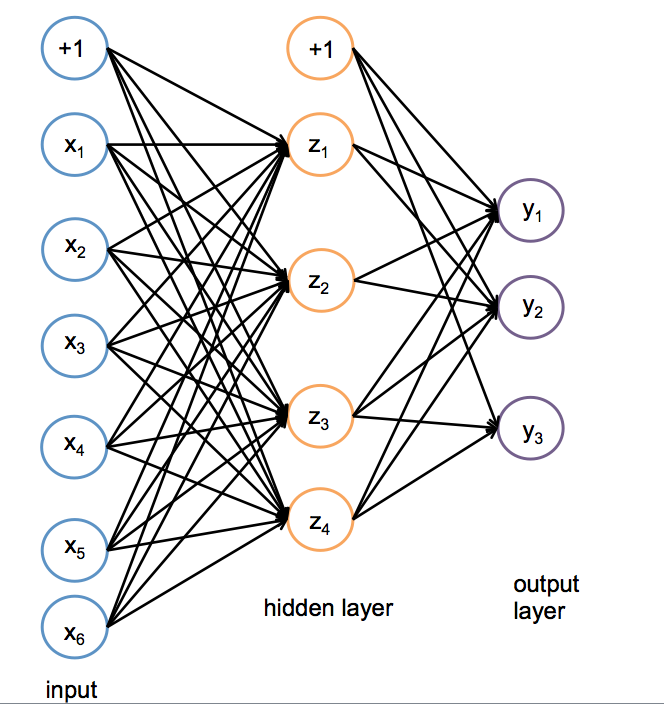
\includegraphics[trim=0 0.2mm 0  0, clip, scale=0.7]{figures/oneHL6.png}
        \caption{A One Hidden Layer Neural Network}
        \label{fig:oneHL}
    \end{figure}

\subsubsection*{\textbf{Network Overview}}
Consider the neural network with one hidden layer shown in Figure \ref{fig:oneHL}. The input layer consists of 6 features $\xv = [x_1,...,x_6]^T$, the hidden layer has 4  nodes $\zv = [z_1,...,z_4]^T$, and the output layer is a probability distribution $\yv = [y_1, y_2, y_3]^T$ over 3 classes. We also add a bias to the input, $x_0 = 1$ and the hidden layer $z_0 = 1$, both of which are fixed to $1$.


We adopt the following notation:
\begin{enumerate}
    \item Let {$\boldsymbol{\alpha}$} be the matrix of weights from the inputs to the hidden layer.
    \item Let {$\boldsymbol{\beta}$} be the matrix of weights from the hidden layer to the output layer.
    \item Let {${\alpha_{j,i}}$} represents the weight going \textit{to} the node $z_j$ in the hidden layer \textit{from} the node $x_i$ in the input layer (e.g. $\alpha_{1,2}$ is the weight from $x_2$ to $z_1$)
    \item Let {${\beta}_{k,j}$} represents the weight going \textit{to} the node $y_k$ in the output layer \textit{from} the node $z_j$ in the hidden layer.
    \item We will use a \emph{sigmoid activation function ({$\sigma$})} for the hidden layer and a \emph{softmax} for the output layer. 
\end{enumerate}

\subsubsection*{\textbf{Network Details}}
Equivalently, we define each of the following. 

The input:
\begin{align}
\xv=[x_1,x_2,x_3,x_4,x_5,x_6]^T
\end{align}

Linear combination at the first (hidden) layer:
\begin{equation}
a_j= \alpha_{j, 0} + \sum_{i=1}^6 \alpha_{j,i}x_i,\quad j \in \{1,\ldots,4\}
\end{equation}

Activation at the first (hidden) layer:
\begin{align}
z_j &= \sigma(a_j) = \frac{1}{1+\exp(-a_j)},\quad  j \in \{1,\ldots,4\}
\end{align}

Linear combination at the second (output) layer:
\begin{equation}
b_k = \beta_{k, 0} + \sum_{j=1}^4 \beta_{k,j}z_j,\quad  k \in \{1,\ldots,3\}
\end{equation}

Activation at the second (output) layer:
\begin{equation}
\hat{y}_k = \frac{\exp(b_k)}{\sum\limits_{l=1}^3 \exp(b_l)},\quad  k \in \{1,\ldots,3\}
\end{equation}

Note that the linear combination equations can be written equivalently as the product of the weight matrix with the input vector. We can even fold in the bias term $\alpha_0$ by thinking of $x_0 = 1$, and fold in $\beta_0$ by thinking of $z_0 = 1$.

\subsubsection*{\textbf{Loss}}

We will use cross entropy loss, $\ell(\hat{\yv},\yv)$. If $\yv$ represents our target (true) output, which will be a \textbf{one-hot vector} representing the correct class, and $\hat{\yv}$ represents the output of the network, the loss is calculated as:
\begin{equation}
   \ell(\hat{\yv},\yv) = - \sum_{k=1}^3 y_k \log(\hat{y}_k)
\end{equation}

\subsubsection*{\textbf{Prediction}}
When doing prediction, we will predict the \textbf{$\argmax$} of the output layer. For example, if $\hat{\yv}$ is such that $\hat{y}_1=0.3,~ \hat{y}_2=0.2,~ \hat{y}_3=0.5$ we would predict class 3 for the input $\xv$. If the true class from the training data $\xv$ was $2$ we would have a \textbf{one-hot vector} $\yv$ with values $y_1=0$,~ $y_2=1$,~ $y_3=0$.
    
\begin{enumerate} 
\item 
     We initialize the weights as:
\begin{center}
$$\boldsymbol{\alpha}=
    \begin{bmatrix}
    1 & 2 & -3 & 0 & 1 & -3 \\
    3 & 1 & 2 & 1 & 0 & 2 \\
    2 & 2 & 2 & 2 & 2 & 1 \\
    1 & 0 & 2 & 1 & -2 & 2
    \end{bmatrix}$$
$$\boldsymbol{\beta}=
    \begin{bmatrix}
    1 & 2 & -2 & 1 \\
    1 & -1 & 1 & 2 \\
    3 & 1 & -1 & 1
    \end{bmatrix}
$$
\end{center}
    
And weights on the bias terms (${\alpha}_{j,0}$ and ${\beta}_{k,0})$ are initialized to 1.
    
    You are given a training example $\xv^{(1)}=[1,1,0,0,1,1]^T$ with label class 2, so $\yv^{(1)}=[0,1,0]^T$. Using the initial weights, run the feed forward of the network over this training example (without rounding during the calculation) and then answer the following questions. 
    %In your responses, round to four decimal places---if the answer is an integer you need not include trailing zeros. 
    
    \begin{enumerate}
        \item What is the value of $a_1$?
        
        \begin{tcolorbox}

        \end{tcolorbox}
        
        
        \item What is the value of $z_1$?
        
        \begin{tcolorbox}

        \end{tcolorbox}
        
        \item What is the value of $a_3$?
        
        \begin{tcolorbox}

        \end{tcolorbox}
    
        
        \item What is the value of $z_3$?
        
        \begin{tcolorbox}

        \end{tcolorbox}
        
        \item What is the value of $b_2$?
        
        \begin{tcolorbox}

        \end{tcolorbox}
        
        
        \item What is the value of $\hat{y}_2$?
        
        \begin{tcolorbox}

        \end{tcolorbox}

        \item Which class value we would predict on this training example?
        
        \begin{tcolorbox}

        \end{tcolorbox}
        

        \item What is the value of the total loss on this training example?
        
        \begin{tcolorbox}

        \end{tcolorbox}
        
    \end{enumerate}
    
    \clearpage
\item Now use the results of the previous question to run backpropagation over the network and update the weights. Use the learning rate $\eta=1$. 
    
    During your backpropagation calculations, \textbf{DON'T} do any rounding. Then answer the following questions: (in your final responses round to four decimal places)
    
     \begin{enumerate}
        \item What is the updated value of ${\beta}_{2,1}$?
        
        \begin{tcolorbox}

        \end{tcolorbox}
        
        
        \item What is the updated weight of the hidden layer bias term applied to $y_1$ (i.e. ${\beta}_{1,0}$)?
        
        \begin{tcolorbox}

        \end{tcolorbox}
        
        \item What is the updated value of ${\alpha}_{3,4}$?
        
        \begin{tcolorbox}

        \end{tcolorbox}
        
        
        \item If we ran backpropagation on this example for a large number of iterations and then ran feed forward over the same example again, which class would we predict?
        
        \begin{tcolorbox}

        \end{tcolorbox}

    \end{enumerate}

\clearpage
\item Let us now introduce regularization into our neural network. For this question, we will incorporate L2 regularization into our loss function $\ell(\hat{\yv},\yv)$, with the parameter $\lambda$ controlling the weight given to the regularization term. 
\begin{enumerate}
    \item Write the expression for the regularized loss function of our network after adding L2 regularization (\textbf{Hint:} Remember that bias terms should not be regularized!) 
    \begin{tcolorbox}

        \end{tcolorbox}
        
        
    \item Compute the regularized loss for training example $\xv^{(1)}$ (assume $\lambda$ = 0.01 and use the weights before backpropagation)
     \begin{tcolorbox}

        \end{tcolorbox}
        
    
     \item For a network which uses the regularized loss function, write the gradient update equation for $\alpha_{j,i}$ . You may use $\frac{\partial \ell(\hat{\yv},\yv)}{\partial \alpha_{j,i}}$ to denote the gradient update w.r.t non-regularized loss and $\eta$ to denote the learning rate.
    \begin{tcolorbox}

        \end{tcolorbox}
    
    
   % \clearpage
    
    \item Based on your observations from previous questions, \textbf{select all statements which are true}:  (\textbf{Hint:} Use ``$\$\backslash$blacksquare$\$$'' ($\blacksquare$) to indicate your choice(s).)
    \begin{list}{}
    \item $\square$ The non-regularized loss is always higher than the regularized loss 
    \item $\square$ As weights become larger, the regularized loss increases faster than non-regularized loss
    \item $\square$ On adding regularization to the loss function, gradient updates for the network become larger
    \item $\square$ When using large initial weights, weight values decrease more rapidly for a network which uses regularized loss 
    \item $\square$ None of the above
\end{list}

    
\end{enumerate}
 

\end{enumerate}        
    \end{Q_nosol}
    




\begin{Q}
    \textbf{\Large Implementing Convolutional Neural Networks.}

    In this problem, you will use convolutional neural networks
    to learn to classify handwritten digits.  The digits will
    be encoded as 8x8 matrices.  The layers of your neural
    network should be:
    \begin{itemize}
        \item A 2D convolutional layer with 1 input channel and 8 output channels, with a kernel size of 3
        \item A 2D maximimum pooling layer, with kernel size 2
        \item A 2D convolutional layer with 8 input channels and 4 output channels, with a kernel size of 3
        \item A fully connected (torch.nn.Linear) layer with 4 inputs and 10 outputs
    \end{itemize}
    Apply the ReLU activation function to the output
    of each of your convolutional layers before inputting them
    to your next layer.  For both of the convolutional layers
    of the network, use the default settings parameters
    (stride=1, padding=0, dilation=1, groups=1, bias=True).

    \begin{enumerate}
        \item Implement the class \texttt{DigitsConvNet}.  Please refer to the dosctrings in hw2.py for details.
        
        \textbf{Library routines:} \texttt{torch.nn.Conv2d, torch.nn.MaxPool2D, and torch.nn.Linear.}
        \item Implement \texttt{fit\_and\_evaluate} for use in
            the next several parts. The utility functions \texttt{train\_batch} and \texttt{epoch\_loss} will be useful. See the docstrings in hw2.py and hw2\_util.py for details.
            
            \textbf{Library routines:} \texttt{torch.no\_grad.}
            
        \item Fit a \texttt{DigitsConvNet} on the train dataset
            from \texttt{torch\_digits} in hw2\_util.py.  Use \texttt{torch.nn.CrossEntropyLoss} as the loss function and \texttt{torch.optim.SGD} as the optimizer with learning rate 0.005 and no momentum. Train your model for 30 epochs with a
            batch size of 1.  Keep track of your training and test loss for part (e).
            
            \textbf{Library routines:} \texttt{torch.optim.SGD, torch.nn.CrossEntropyLoss, torch.save.}
        \item Fit another \texttt{DigitsConvNet} with \texttt{torch.nn.CrossEntropyLoss} and \texttt{torch.optim.SGD} with learning rate 0.005, no momentum, and a batch size of 1 for 30 epochs.  This time we will adjust the learning rate so that it decreases
            at each epoch.  Recall the gradient descent update step
            $$\vw_{i+1} = \vw_i - \eta_i \nabla_{\vw} \cL(\vw_i).$$
            where $\cL$ is the loss function and $i$ is the step index. We will update the learning rate only at the end of each epoch. Therefore, $\eta_{i+1} \coloneqq \eta_i$ within each epoch and $\eta_{i+1} = \gamma \cdot \eta_i$ at the end of each epoch.  You should use             \texttt{torch.optim.lr\_scheduler.ExponentialLR}.  Use a decay rate of $\gamma=0.95$ and
            start the learning rate at 0.005. You may find it useful to temporarily modify your \texttt{fit\_and\_evaluate} function to include a scheduler for this part. Keep track of your training and test loss for part (e). 
            
            \textbf{Library routines:} \texttt{torch.optim.lr\_scheduler.ExponentialLR, torch.nn.CrossEntropyLoss, torch.save.}
        \item Fit a third \texttt{DigitsConvNet}, again with \texttt{torch.nn.CrossEntropyLoss} and \texttt{torch.optim.SGD}
            with learning rate 0.005 and no
            momentum for 30 epochs.  However, this time use a batch size of
            16. 
            
            \vspace{1.5mm}\textbf{Plot the epochs vs training and test losses for parts (c), (d), and (e)} (you should have six plots on the same figure, include this figure in your written submission).  For plot legend, please name the two plots in (c) as "train batch = 1", "test batch = 1", (d) as "train decayed\_lr = 1", "test decayed\_lr = 1", (e) as "train batch = 16", "test batch = 16".
            
            \vspace{1.5mm}\textbf{You do **not** need to include the plot generation code in your code submission.}
            
            \vspace{1.5mm}Include the figure and your assessment of the impact the exponentially decayed learning rate has
            on training speed (the behavior of the loss, not CPU time).  Additionally, comment on the
            impact that increasing the batch size has on loss. 
            
            \vspace{1.5mm}In your report, you may leave parts (c) and (d) blank and include all comments in part (e). Note that it is normal to get different plots for separate runs as PyTorch randomly initializes the weights. We added `torch.manual\_seed(0)' in the coding template to make everyone's plot look similar.
            
            \vspace{1.5mm}\textbf{Library routines:} \texttt{torch.optim.SGD, torch.nn.CrossEntropyLoss, plt.plot, plt.legend, torch.load.}
    \end{enumerate}\end{Q}
    \begin{tcolorbox}

    \end{tcolorbox}


 
    
\end{enumerate}

\newpage
\bibliography{hw2}
\end{document}
